\documentclass{fkssolpub}

\usepackage[czech]{babel}
\usepackage{fontspec}
\usepackage{fkssugar}
\usepackage{amsmath}
\usepackage{graphicx}

\author{Ondřej Sedláček}
\school{Gymnázium Oty Pavla} 
\series{3p}
\problem{2} 

\begin{document} 

Níže můžete vidět příklad kružnic, které splňují zadání. Skládá se z šesti kružnic,
z nichž vnějšek tvoří tři kružnice a vnitřek tvoří také tři kružnice, které získáme
stejnolehlostí se středem v průsečíků tečen procházející dotykovými body vnějších kružnic
a takovými koeficienty, aby se vnitřní kružnice dotýkaly vnějších.

\begin{figure}[h!]
  \centering
  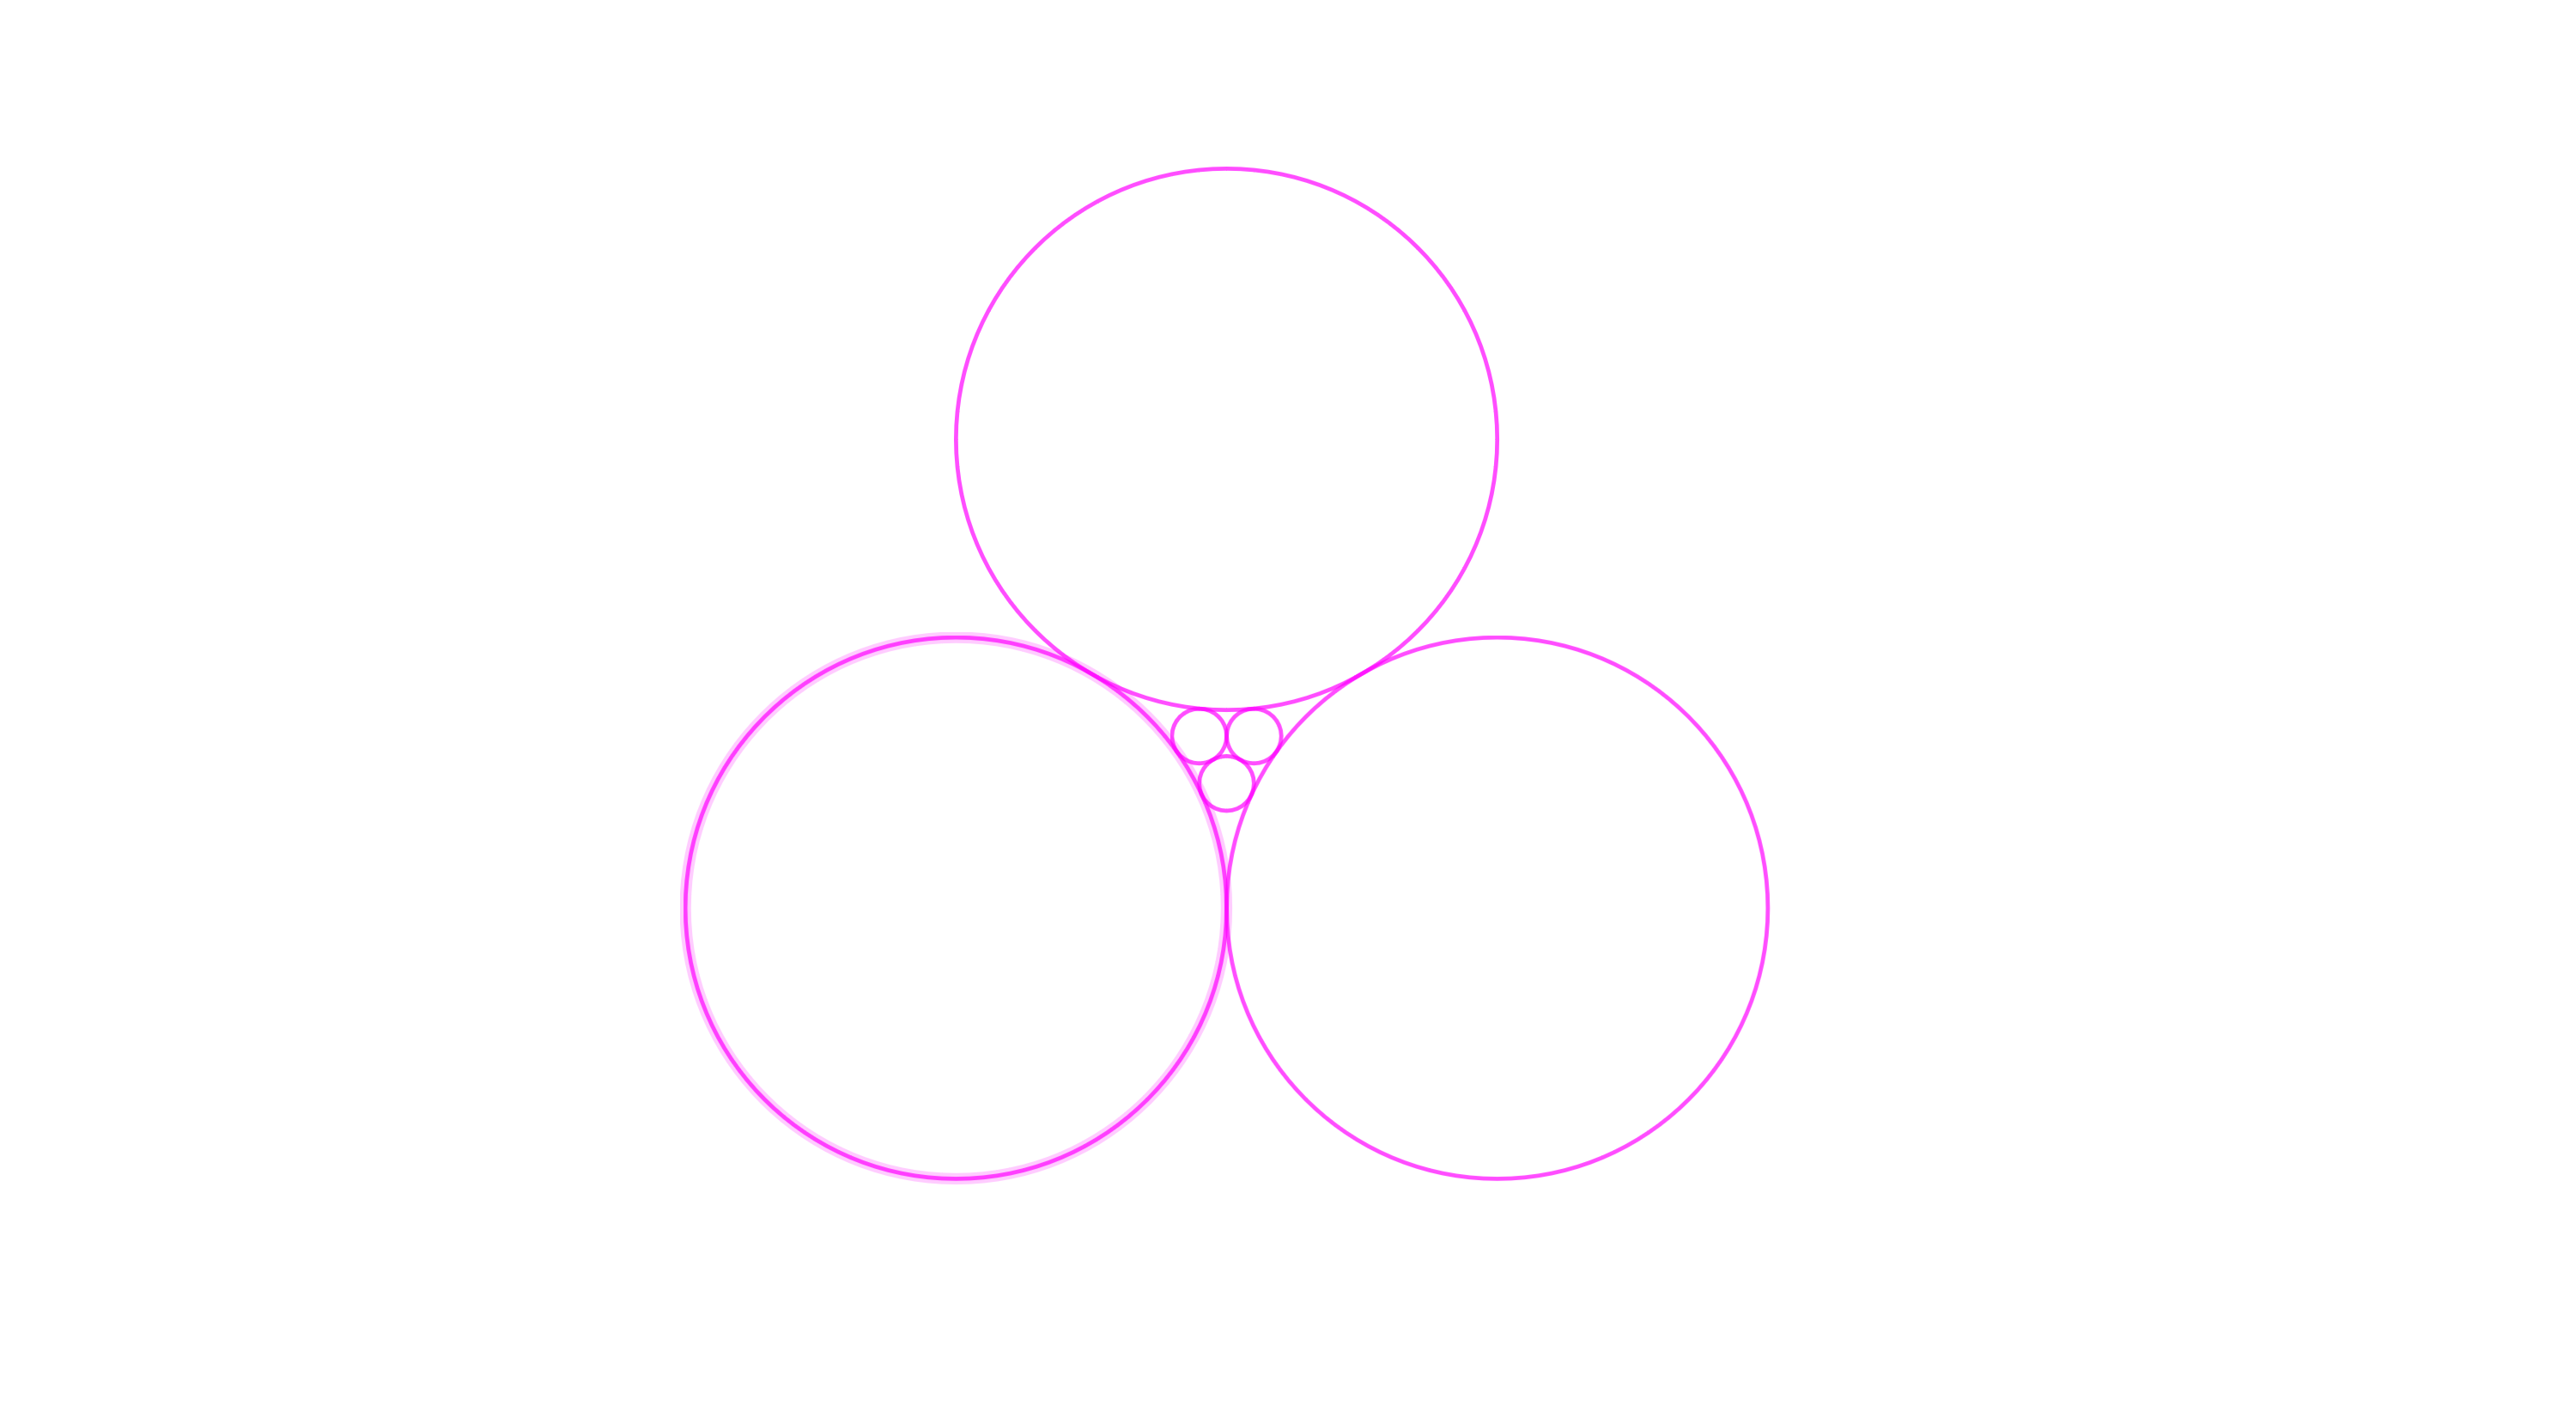
\includegraphics{2-fig.png}
  \caption{Růžové kružnice splňující zadání}
\end{figure}

\end{document}
